\documentclass[12pt,a4paper]{article}
\usepackage[T1]{fontenc}
\usepackage[utf8]{inputenc}
\usepackage[brazil]{babel}
\usepackage{geometry}
\usepackage{graphicx}
\usepackage{booktabs}
\usepackage{tabularx}
\usepackage{float}
\usepackage{enumitem}
\usepackage{xcolor}
\usepackage[hidelinks]{hyperref}

\geometry{margin=2.2cm}
\setlength{\parindent}{0pt}
\setlength{\parskip}{0.5em}
\definecolor{ParetolabGreen}{HTML}{28624D}

\title{\textbf{Relatório de Tomada de Decisão}\\[0.4em]
\large Instância TSP BIOBJETIVO}
\author{Execução \texttt{run\_cc44931f62fb4f6f9de63261fb58c9fb}}
\date{}

\begin{document}
\maketitle

\section*{Contexto da análise}

Este relatório foi gerado a partir dos dados persistidos no PostgreSQL da instância
\texttt{inst\_1f56c2c435ad4faabf7beeefc811ac7a} e da execução concluída
\texttt{run\_cc44931f62fb4f6f9de63261fb58c9fb}.

\begin{itemize}[leftmargin=*]
  \item Instância: \texttt{TSP BIOBJETIVO}
  \item Nós da instância: 250
  \item Algoritmo: \texttt{neuro-lkh}
  \item Execução: 50 iterações e 5 repetições
  \item Semente: \texttt{4180680559}
  \item Soluções persistidas: 250
  \item Marcas não dominadas acumuladas por rodada: 26
  \item Fronteira aproximada global, recalculada sobre todas as soluções: 8 pontos
  \item Alternativas incluídas no ranking AHP persistido: 8
\end{itemize}

A execução produziu uma aproximação da fronteira de Pareto, não uma fronteira ótima garantida.

\section{Processo de tomada de decisão}

O processo combina duas etapas.

\subsection{Otimização e análise de robustez}

\begin{itemize}[leftmargin=*]
  \item As rotas foram avaliadas em 5.000 cenários Monte Carlo.
  \item Semente da simulação: 42.
  \item Coeficiente de variação dos tempos dos arcos: 20\%.
  \item Correlação regional intra-arco: 30\%.
  \item Convenção dos tempos aleatórios: preservação da média nominal.
  \item Avaliação dividida em 8 regiões espaciais obtidas por k-means nos pontos médios dos arcos.
\end{itemize}

\subsection{Priorização multicritério pelo AHP}

\begin{itemize}[leftmargin=*]
  \item Foram usados quatro critérios: distância, tempo nominal, emissão de CO2 e Min-Max Regret.
  \item O decisor realizou comparações par a par na escala de Saaty.
  \item Os pesos dos critérios foram obtidos pelo vetor de prioridades da matriz.
  \item As alternativas receberam pesos locais normalizados pelo desempenho em cada critério.
  \item A pontuação global foi calculada pela soma do peso de cada critério multiplicado pelo peso local da alternativa.
\end{itemize}

\subsection{Critérios de preferência}

\begin{table}[H]
\centering
\begin{tabularx}{\textwidth}{>{\raggedright\arraybackslash}p{3cm} >{\raggedleft\arraybackslash}p{2cm} X}
\toprule
\textbf{Critério} & \textbf{Peso global} & \textbf{Preferência observada} \\
\midrule
Tempo nominal & 44,20\% & Critério predominante \\
Min-Max Regret & 25,71\% & Forte importância relativa à distância \\
Emissão de CO2 & 24,65\% & Importância intermediária \\
Distância & 5,44\% & Critério com menor peso \\
\bottomrule
\end{tabularx}
\caption{Pesos dos critérios no AHP.}
\end{table}

\begin{table}[H]
\centering
\begin{tabular}{lr}
\toprule
\textbf{Comparação par a par} & \textbf{Julgamento} \\
\midrule
Distância em relação ao tempo & 1/9 \\
Distância em relação ao CO2 & 1/3 \\
Distância em relação ao Min-Max Regret & 1/5 \\
Tempo em relação ao CO2 & 3 \\
Tempo em relação ao Min-Max Regret & 1 \\
CO2 em relação ao Min-Max Regret & 2 \\
\bottomrule
\end{tabular}
\caption{Julgamentos persistidos no banco.}
\end{table}

O decisor considerou o \textbf{tempo nominal muito mais importante que a distância},
deu peso moderado ao tempo em relação ao CO2 e tratou tempo e Min-Max Regret como
igualmente importantes.

\subsection{Validade dos julgamentos}

A matriz dos quatro critérios produziu:

\begin{itemize}[leftmargin=*]
  \item Autovalor máximo $\lambda_{\max}$: 4,3308
  \item Índice de consistência: 0,1103
  \item Razão de consistência: 12,25\%
\end{itemize}

A razão de consistência excede o limite recomendado de 10\%. Assim, o ranking é
\textbf{provisório} e os julgamentos deveriam ser revisados. A diferença entre a
primeira e a segunda alternativa é pequena o suficiente para tornar essa revisão relevante.

\section{Cenário vencedor}

A alternativa vencedora é \textbf{S6}, identificada no banco como
\texttt{sol\_b0eb4bcb0a684a55bc096fc77518d2da}.

\begin{table}[H]
\centering
\small
\begin{tabularx}{\textwidth}{>{\raggedright\arraybackslash}X r}
\toprule
\textbf{Característica} & \textbf{Valor} \\
\midrule
Posição no ranking AHP & 1 \\
Pontuação AHP & 17,284\% \\
Distância & 1.266,30 km \\
Tempo nominal & 18,50 h \\
Emissão de CO2 & 414,3915 kg \\
CO2 base pela distância & 379,89 kg \\
Excesso por fator de velocidade & 34,5015 kg \\
Fator total de emissão por velocidade & 1,09082 \\
Arcos da rota & 249 \\
Min-Max Regret & 0,0513949 \\
P95 do Min-Max Regret & 0,0651419 \\
Probabilidade de pertencer à fronteira & 73,88\% \\
Frequência de vitória em tempo & 1,96\% \\
Tempo médio simulado & 18,5035 h \\
P95 do tempo & 19,7956 h \\
P99 do tempo & 20,4055 h \\
CVaR95 do tempo & 20,1620 h \\
Desvio-padrão do tempo & 0,7742 h \\
CV do tempo & 4,1842\% \\
Regret médio em tempo & 0,6450 h \\
Regret P95 em tempo & 1,1671 h \\
Contribuição ao hipervolume & 32,0058 \\
\bottomrule
\end{tabularx}
\caption{Características da solução vencedora S6.}
\end{table}

S6 apresenta um compromisso equilibrado entre tempo e robustez. Sua distância é
intermediária entre os extremos da fronteira, seu tempo nominal fica próximo do melhor
extremo de tempo e seu Min-Max Regret é o segundo menor dos oito concorrentes, atrás
apenas de S5.

\begin{figure}[H]
  \centering
  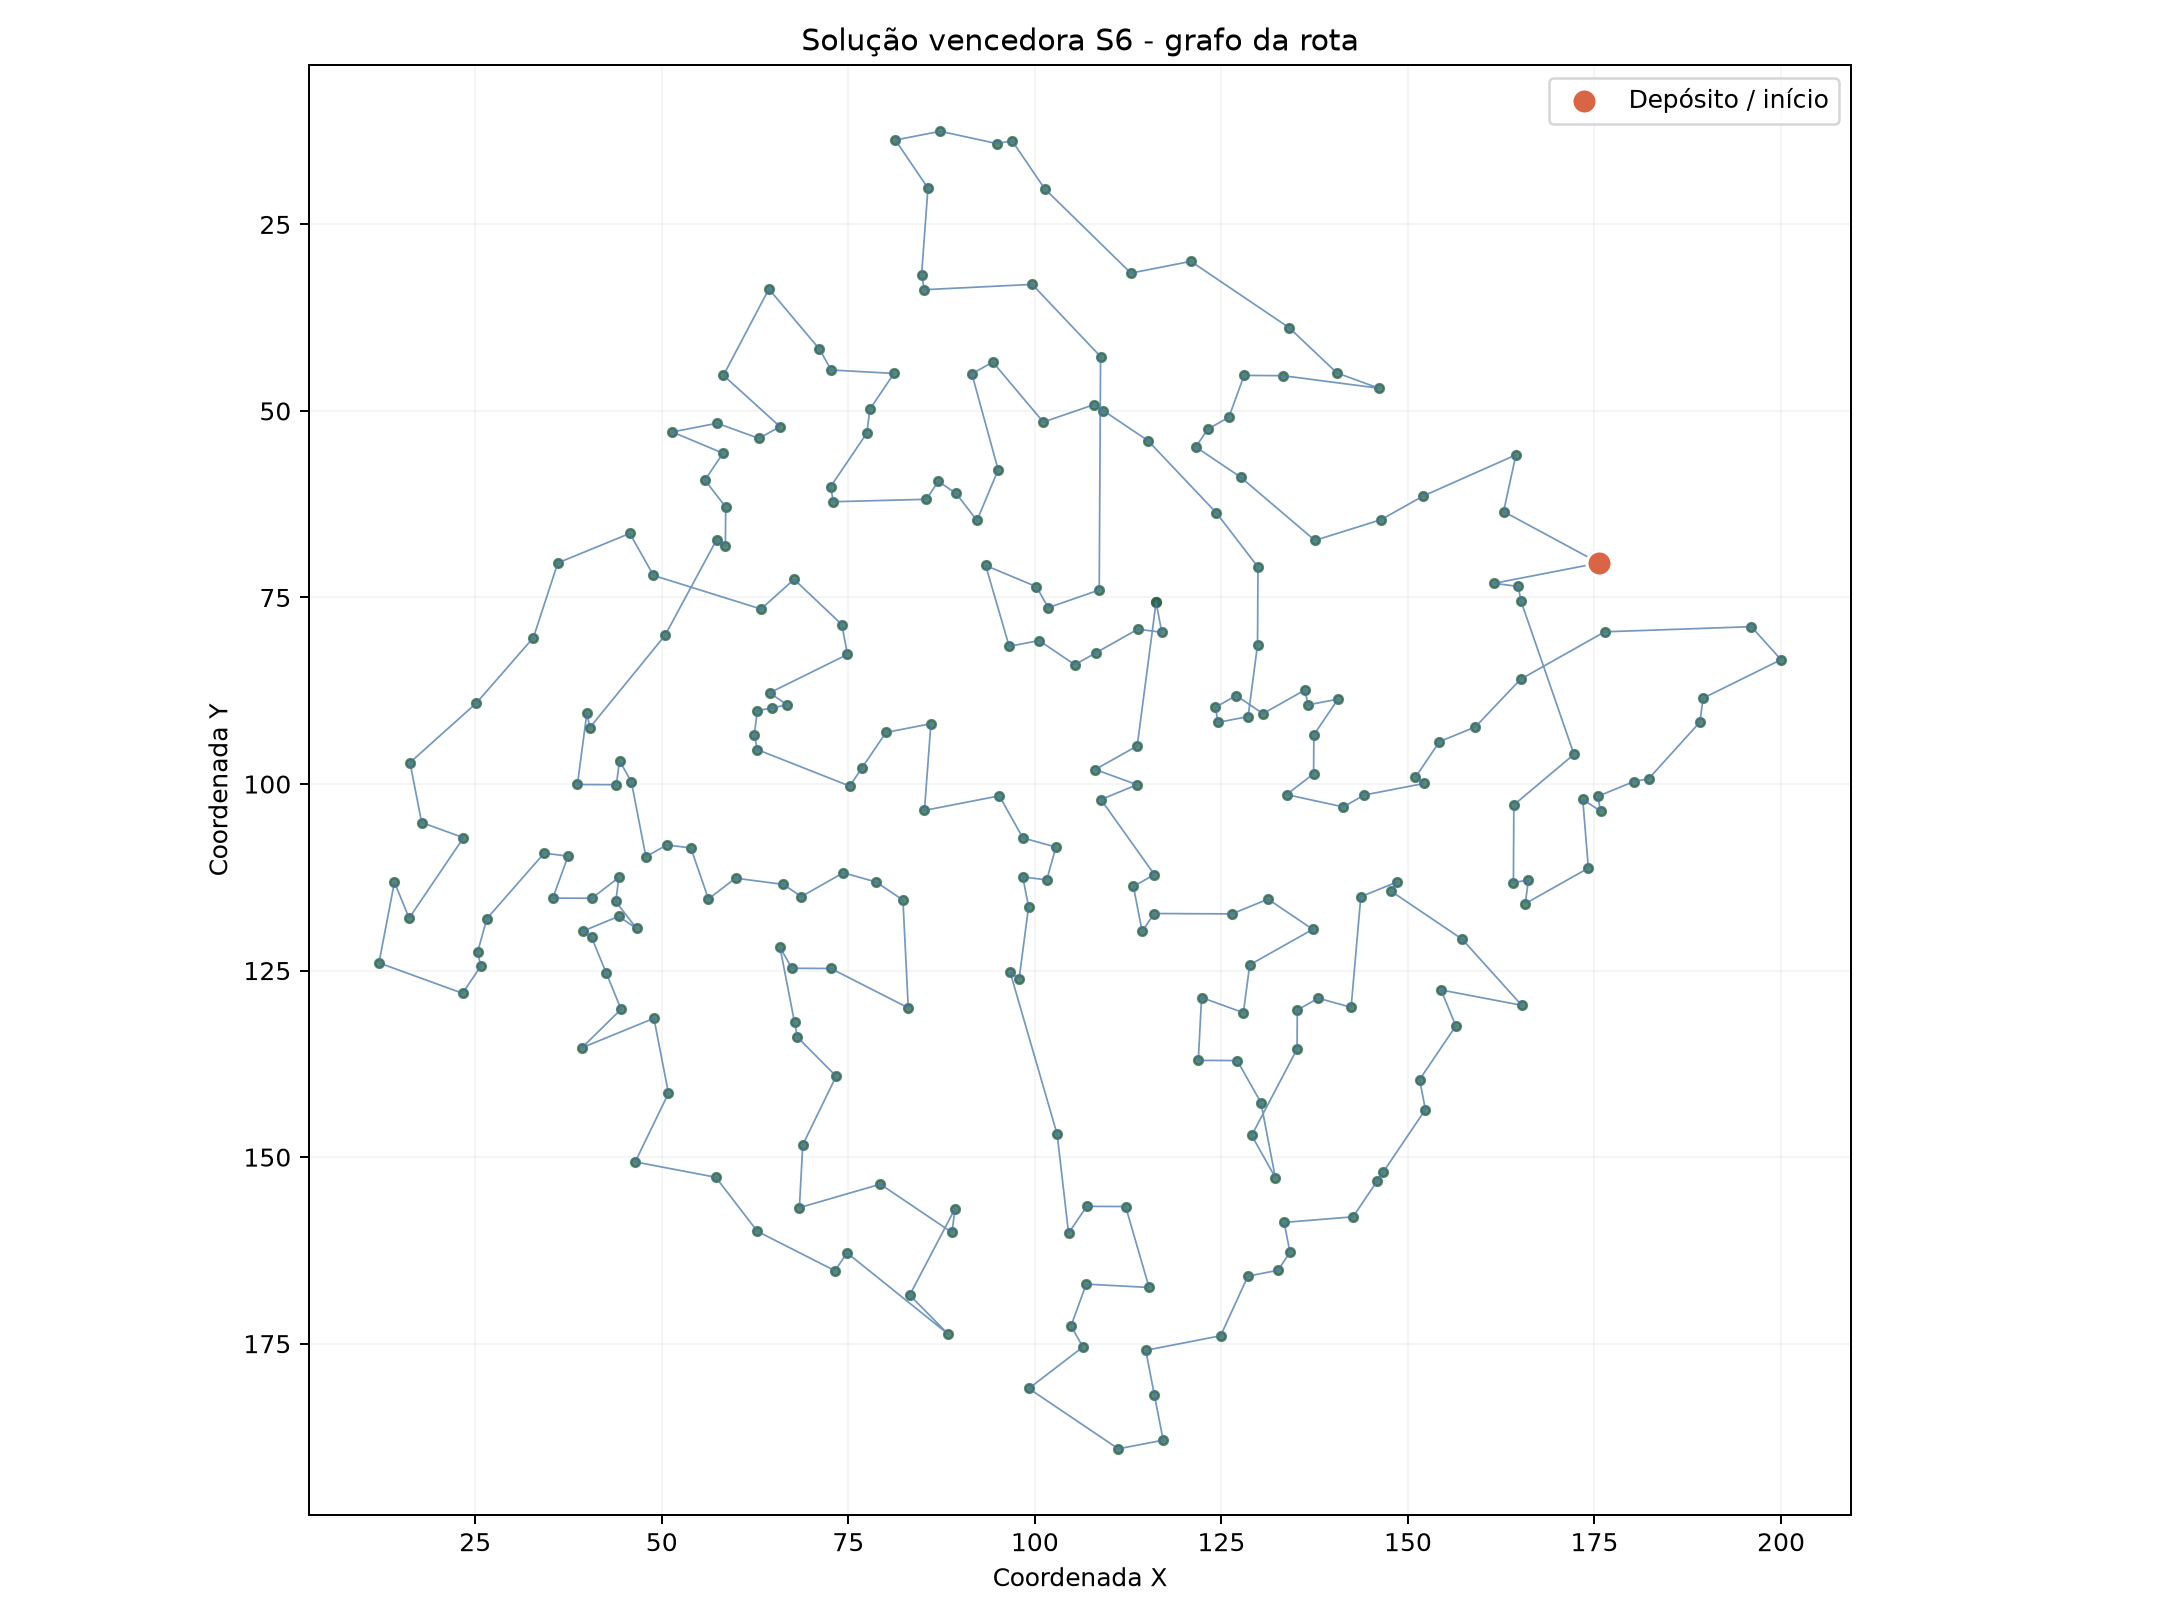
\includegraphics[width=0.82\textwidth]{assets/rota_s6_sem_co2.png}
  \caption{Grafo da solução vencedora S6 sem densidade de CO2.}
\end{figure}

\begin{figure}[H]
  \centering
  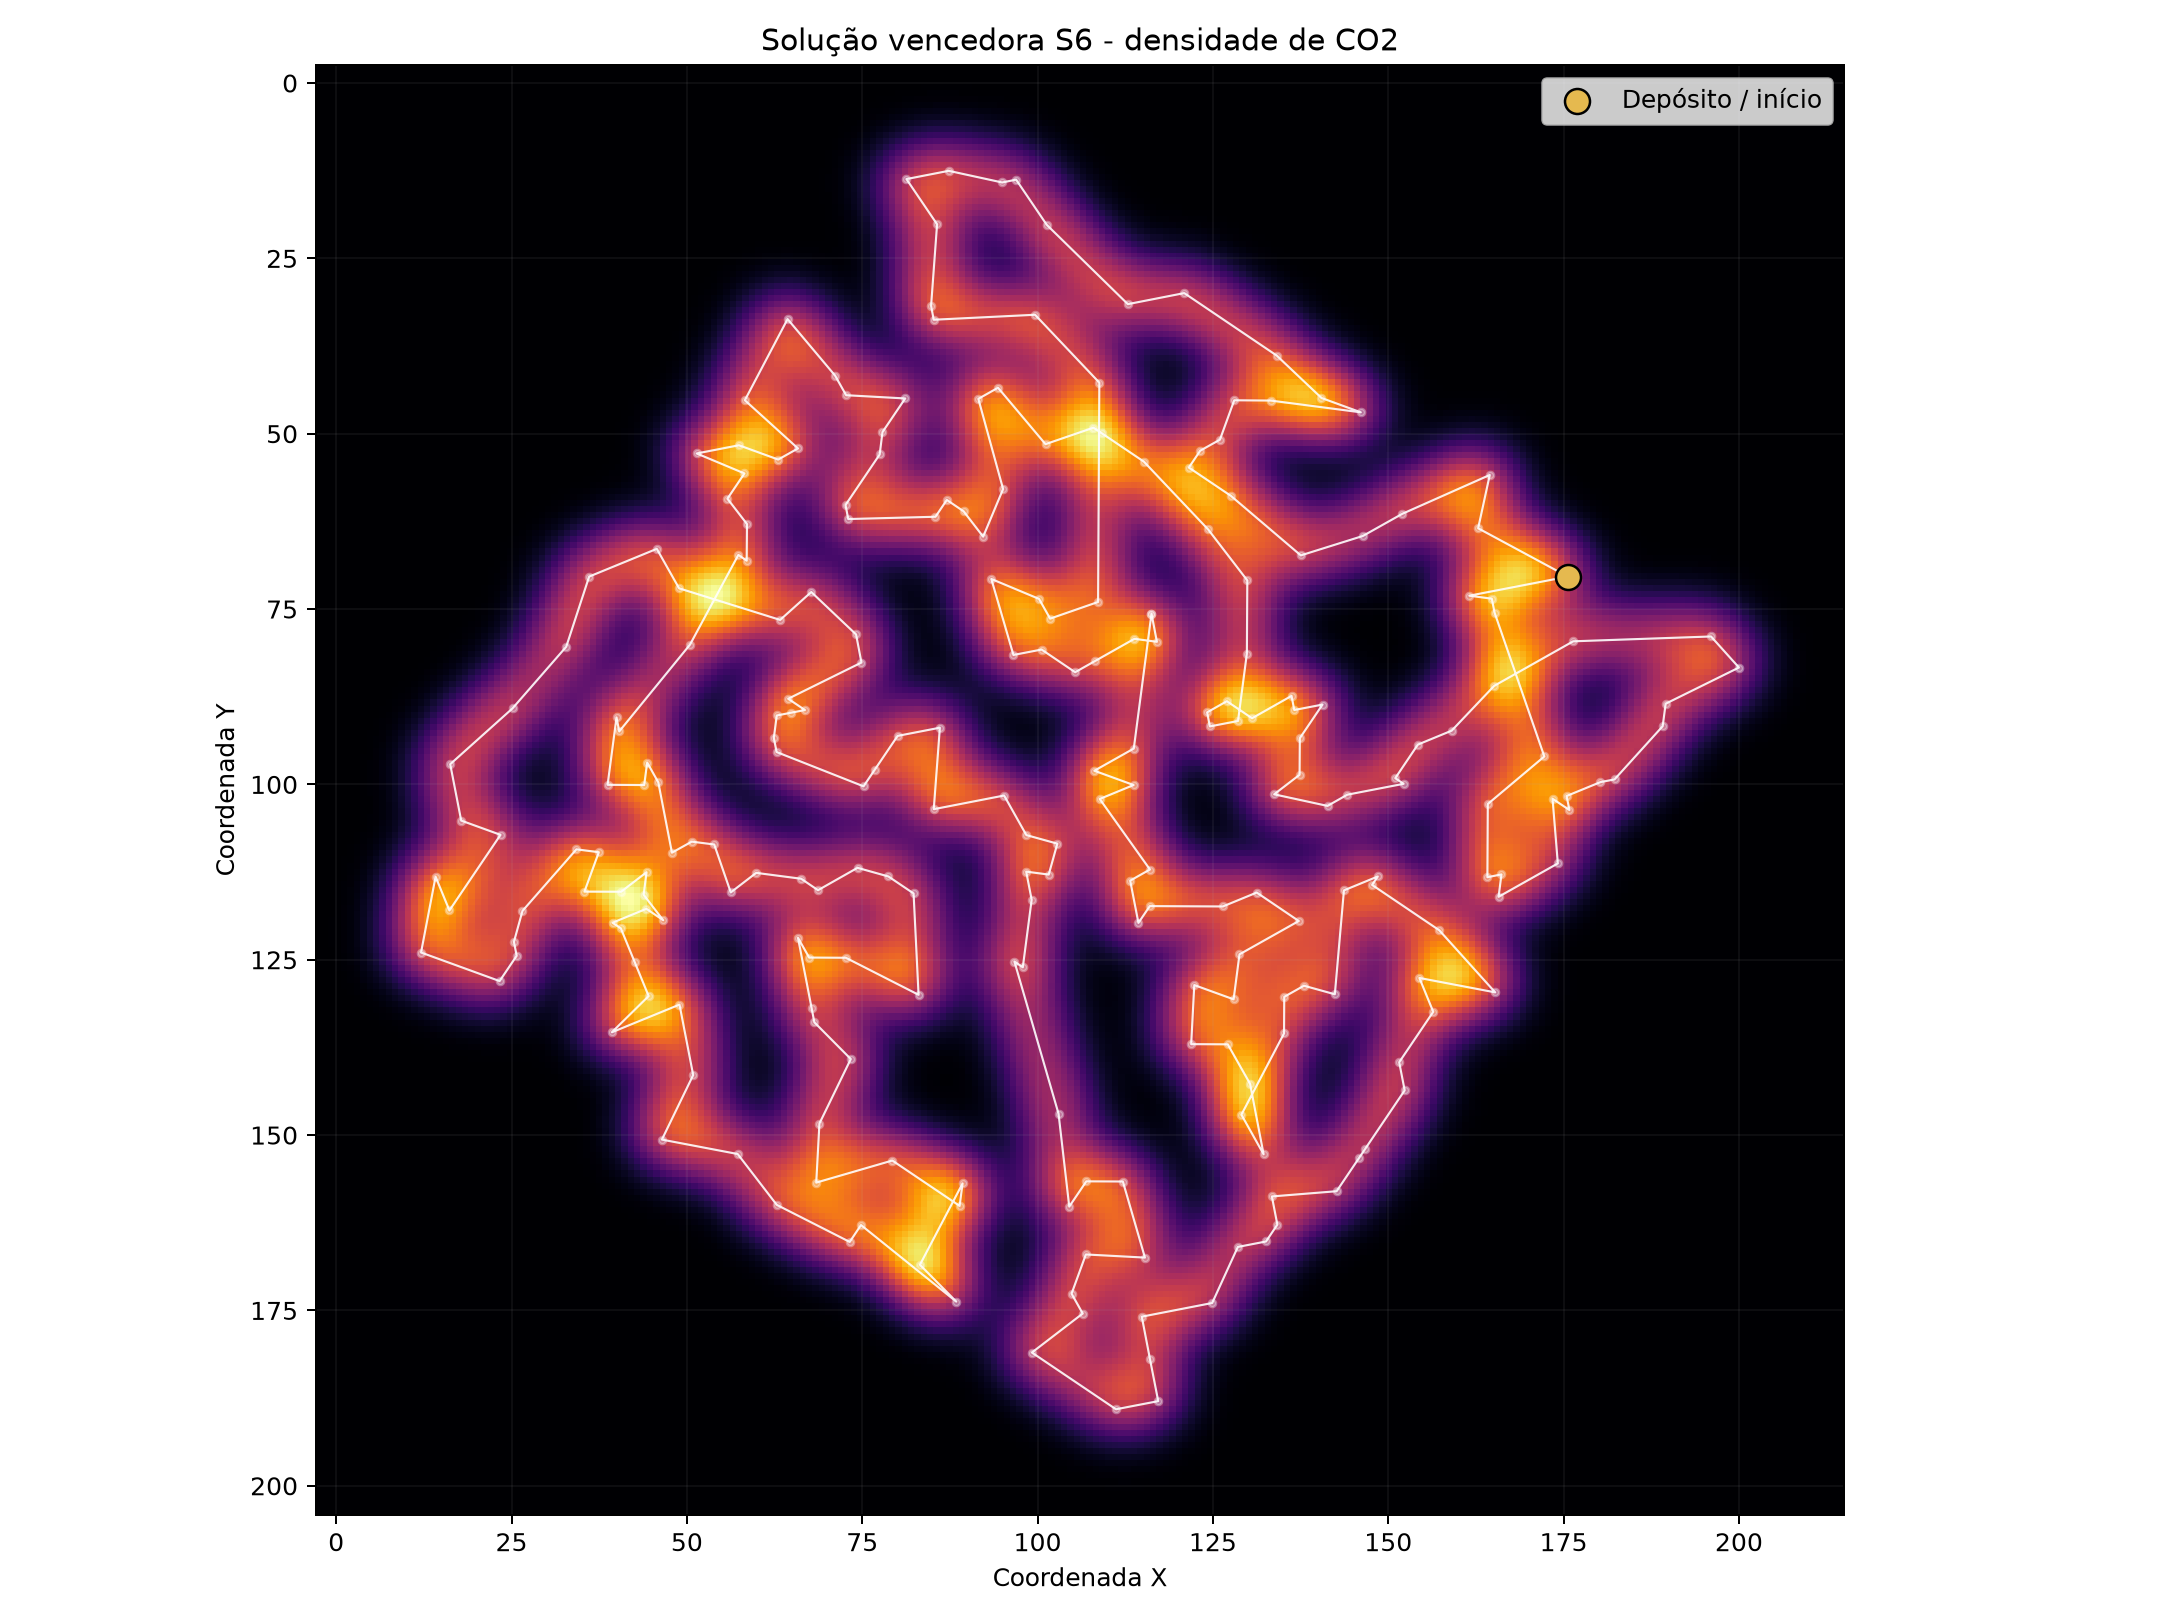
\includegraphics[width=0.82\textwidth]{assets/rota_s6_com_co2.png}
  \caption{Grafo da solução vencedora S6 com densidade de CO2.}
\end{figure}

\section{Comparação dos concorrentes}

\begin{table}[H]
\centering
\small
\begin{tabular}{r l r r r r r r}
\toprule
\textbf{Rank} & \textbf{Solução} & \textbf{Distância} & \textbf{Tempo} &
\textbf{CO2} & \textbf{Min-Max} & \textbf{Prob.} & \textbf{Pontuação} \\
 & & \textbf{(km)} & \textbf{(h)} & \textbf{(kg)} & \textbf{Regret} &
\textbf{fronteira} & \textbf{AHP} \\
\midrule
1 & S6 & 1.266,3 & 18,5 & 414,3915 & 0,0513949 & 73,88\% & 17,2844\% \\
2 & S5 & 1.259,1 & 18,7 & 411,2220 & 0,0478831 & 100,00\% & 17,1933\% \\
3 & S7 & 1.377,2 & 18,1 & 456,5730 & 0,1434739 & 85,10\% & 12,7747\% \\
4 & S4 & 1.258,1 & 20,0 & 410,1105 & 0,1204109 & 95,36\% & 12,7000\% \\
5 & S8 & 1.412,2 & 17,9 & 469,6680 & 0,1725340 & 71,52\% & 11,5058\% \\
6 & S2 & 1.233,8 & 20,7 & 402,5910 & 0,1597029 & 99,82\% & 10,7413\% \\
7 & S3 & 1.257,1 & 20,6 & 412,2990 & 0,1541186 & 60,06\% & 10,4802\% \\
8 & S1 & 1.204,4 & 21,9 & 390,0945 & 0,2266580 & 100,00\% & 7,3204\% \\
\bottomrule
\end{tabular}
\caption{Ranking AHP e características dos concorrentes.}
\end{table}

Os oito itens são as alternativas persistidas no ranking AHP. Todas as oito alternativas
são não dominadas dentro do conjunto considerado pelo ranking. A fronteira aproximada
global contém exatamente 8 pontos: S1, S2, S3, S4, S5, S6, S7 e S8.

\subsection{Características dos concorrentes}

\begin{itemize}[leftmargin=*]
  \item \textbf{S5 --- principal concorrente:} menor Min-Max Regret e pontuação apenas
  0,091 ponto percentual abaixo de S6. Possui probabilidade de pertencer à fronteira de
  100\%, tempo de 18,7 h e CO2 de 411,222 kg.
  \item \textbf{S7:} alternativa com tempo de 18,1 h, mas mais distante e com emissão
  muito maior; seu Min-Max Regret é aproximadamente 2,8 vezes o de S6.
  \item \textbf{S4:} distância próxima à de S6 e menor CO2, porém com tempo nominal de
  20 h e Min-Max Regret maior.
  \item \textbf{S8:} melhor extremo nominal de tempo, com 17,9 h, mas maior distância e
  maior emissão entre os oito concorrentes.
  \item \textbf{S2:} menor distância apenas entre os oito concorrentes, mas tempo nominal
  elevado de 20,7 h.
  \item \textbf{S3:} distância e CO2 próximos de S6, porém tempo nominal de 20,6 h e
  regret maior.
  \item \textbf{S1:} menor distância e menor CO2 absoluto, mas maior tempo nominal,
  21,9 h, e maior Min-Max Regret.
\end{itemize}

\section{Curva de Pareto mapeada}

\subsection{Como a curva foi obtida}

A curva não usa a marcação de dominância calculada separadamente em cada rodada.
Para obter a \textbf{fronteira aproximada global}, foram consideradas as 250 soluções
persistidas da execução e aplicada a relação de dominância sobre a união:

\begin{enumerate}[leftmargin=*]
  \item O objetivo é minimizar distância e tempo.
  \item Uma solução candidata é dominada quando existe outra solução com distância não
  maior e tempo não maior, sendo melhor em pelo menos um desses objetivos.
  \item Uma solução pertence à curva somente quando não é dominada por nenhuma outra
  solução da união.
  \item Os pontos resultantes foram ordenados pela distância.
\end{enumerate}

Nesse método, a curva aproximada global contém \textbf{8 soluções}. Nenhum desses pontos
domina outro ponto da própria fronteira.

As 26 marcas \texttt{non\_dominated} eram a soma dos pontos não dominados dentro de cada
rodada. Esse conjunto acumulado não corresponde à fronteira global: pode conter soluções
dominadas por alternativas encontradas em outras rodadas.

\begin{figure}[H]
  \centering
  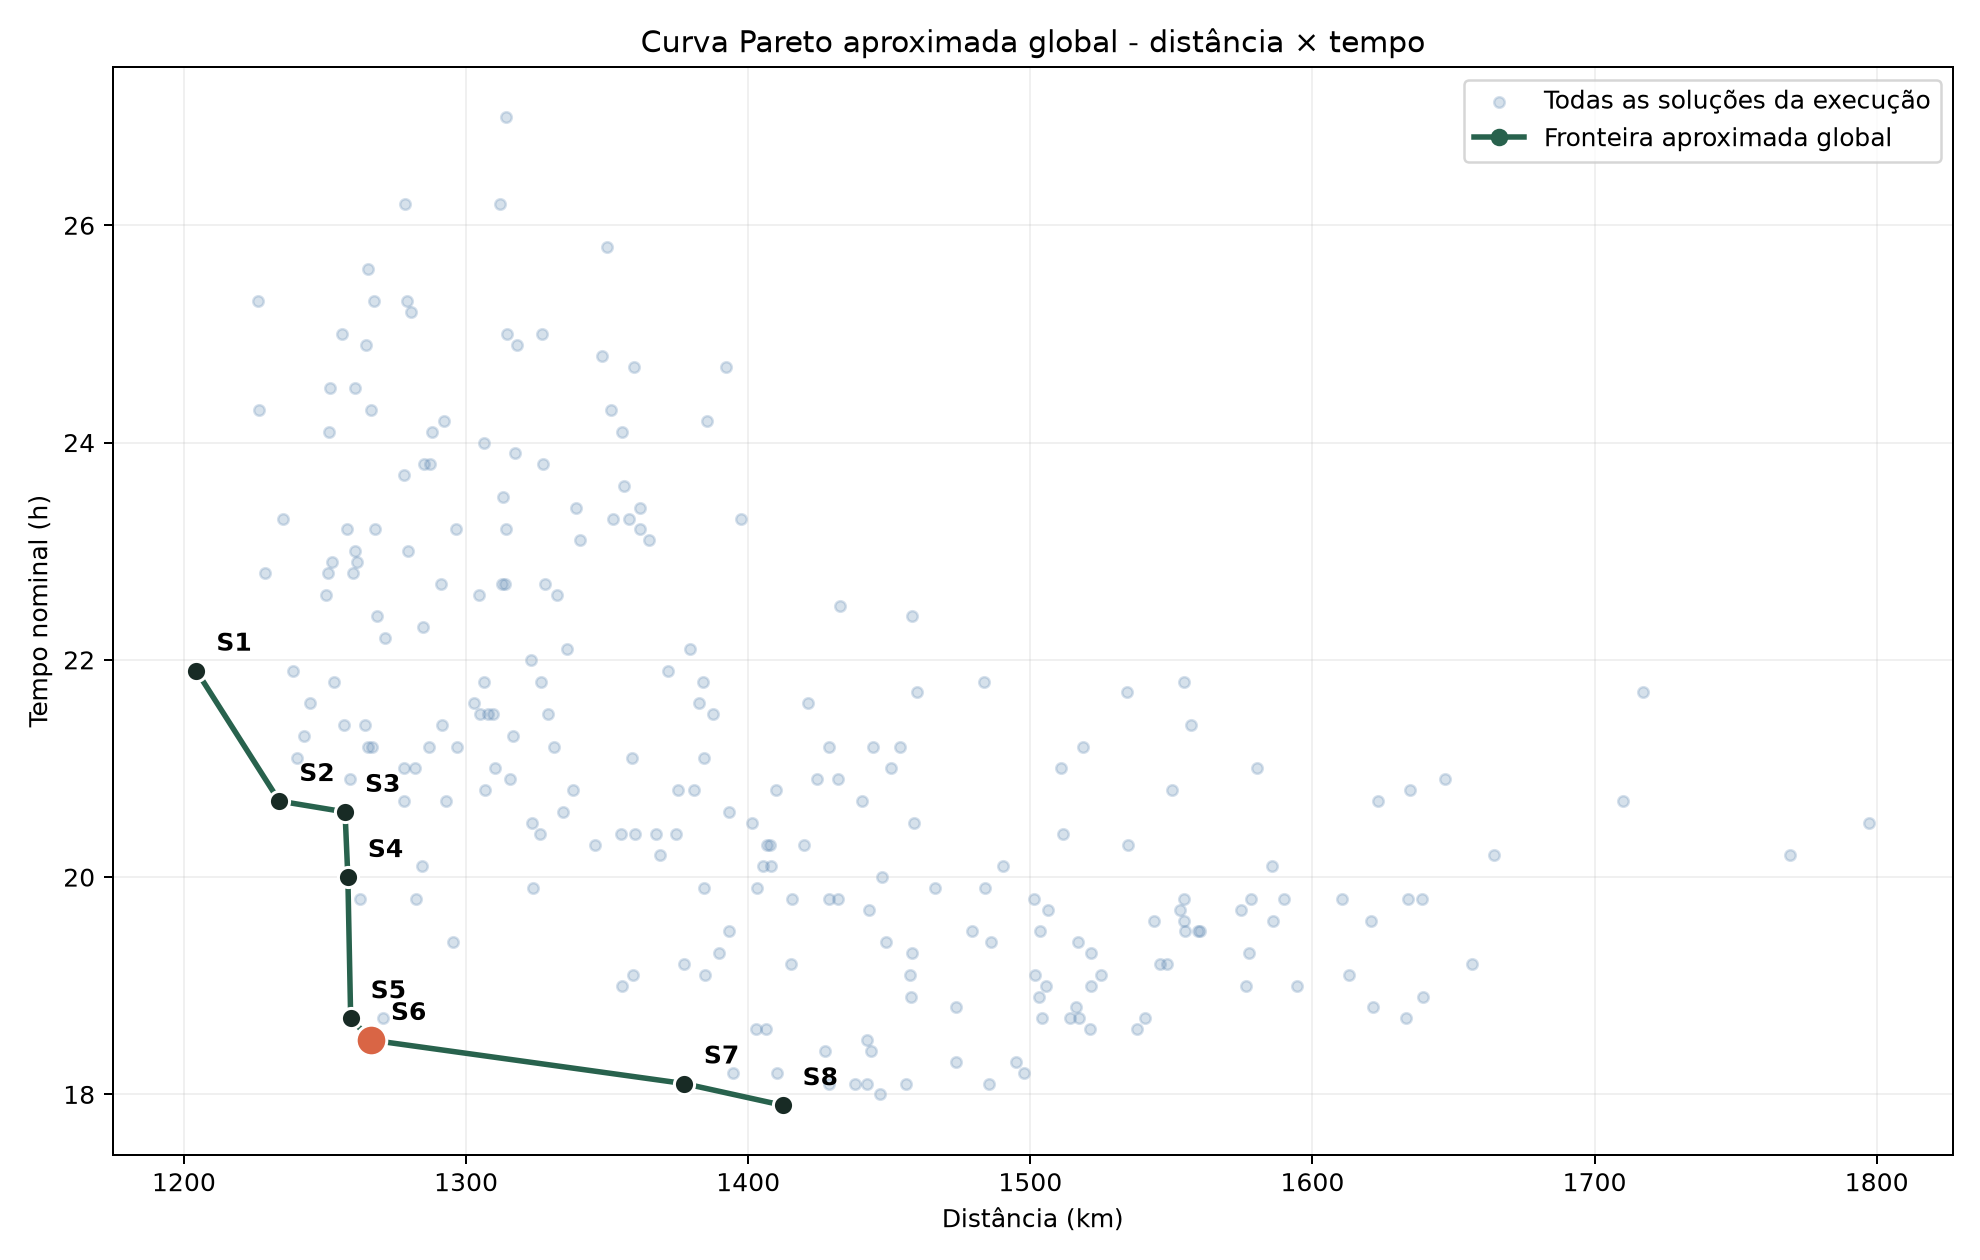
\includegraphics[width=0.88\textwidth]{assets/curva_pareto_mapeada.png}
  \caption{Curva Pareto aproximada global --- distância versus tempo.}
\end{figure}

Os extremos aproximados da fronteira são:

\begin{itemize}[leftmargin=*]
  \item Distância mínima: 1.204,40 km, com tempo nominal de 21,90 h.
  \item Tempo mínimo: 17,90 h, com distância de 1.412,20 km.
\end{itemize}

O vencedor S6 está na região intermediária da curva, com 1.266,30 km e 18,50 h.
A proximidade com S5 mostra que os pesos do decisor são decisivos para o primeiro lugar.

\section{Conclusão}

O processo de decisão selecionou \textbf{S6} porque combina tempo nominal baixo,
segundo menor Min-Max Regret e níveis intermediários de distância e emissão.
O resultado não deve ser tratado como definitivo enquanto a razão de consistência
permanecer acima de 10\%. Uma revisão das preferências pode alterar a liderança entre
S6 e S5.

\end{document}
